\documentclass{article}
\usepackage{graphicx, fancyhdr, amsmath}
\usepackage[margin=0.6in, top=1in]{geometry}
\usepackage{float}
\usepackage[absolute, overlay]{textpos}
\usepackage[colorlinks=true, linkcolor=blue]{hyperref}

\pagestyle{fancy}
\fancyhf{}
\renewcommand{\headrulewidth}{0pt}

\fancyhead[L]{
\begin{textblock*}{2cm}(0.3in,0.1in)  % {block width} (x-coordinate, y-coordinate)
    
\includegraphics[width=2cm]{NEW LOGO.png}  % Example image placeholder
\end{textblock*}
}
\fancyhead[R]{Math Success Program, UCLA}
\fancyfoot[R]{Created for the MSP by Asmi Kawatkar}

\fancypagestyle{plain}{
}


\title{Review Sheet: Implicit Differentiation}
\date{}
\author{}

\begin{document}
\maketitle
\vspace{-0.75in}
\section*{Content Review}
\subsection*{Overview}

Implicit differentiation involves trying to take the derivative with respect to a variable that you sometimes 'cannot see'. For instance, if we are given that $y$ is a function of $x$, and we want to find the derivative of $y^2$ with respect to $x$, then:

$$\frac{d}{dx}(y^2) = \frac{d}{dy}(y^2)\cdot \frac{d}{dx}(y) = 2y \cdot \frac{dy}{dx}$$
This is because of the chain rule. 
\\
\textbf{Recall:} The Chain Rule states that
$$\frac{dy}{dx} = \frac{dy}{du}\cdot \frac{du}{dx}$$
\\
Note that the final solution to the problem above contains a term $\frac{dy}{dx}$. This is because we don't explicitly know what $y$ is in terms of $x$, so we cannot simplify this term further. 
\\
However, if it was given that $y = \frac{\sin x}{2}$, for example, then we can simplify $$\frac{dy}{dx} = \frac{d}{dx}\left(\frac{\sin x}{2}\right)$$

\subsection*{Frequently Asked Questions}

\begin{enumerate}
    \item Chain Rule vs Implicit Differentiation?
    \vspace{3pt}
    \newline
    \textbf{Ans}:Implicit Differentiation is a special application of chain rule, where the $\frac{dy}{dx}$ term appears because $y$ is a function of $x$, and by chain rule, we must take the derivative of $y$ with respect to $x$ as well. 

    \item Partial Differentiation vs Implicit Differentiation? \textit{[Ignore this if you haven't come across partial derivatives yet!]}
    \vspace{3pt}
    \newline
    \textbf{Ans}: Partial Differentiation involves holding all remaining the variables constant while differentiating with respect to one of the variables. 
    For example:
    $$\frac{\partial}{\partial x} x^2+y^2 = \frac{\partial}{\partial x} x^2 + \frac{\partial }{\partial x} y^2 = 2x + 0 = 2x$$
    Here, the \textbf{\textit{partial derivative}} of $y^2$ with respect to $x$ is 0, since we pretend that $y^2$ is a constant with respect to $x$ (i.e. a change in $x$ does not cause a change in $y$, and $y$ is not a function of $x$)

    However, in Implicit Differentiation, we assume that $y$ is a function of $x$, so the same expression above would evaluate to:
    $$\frac{d}{dx} x^2 + y^2 = \frac{d}{dx}x^2 +\frac{d}{dx}y^2 = 2x + 2y\frac{dy}{dx}$$

    Note the use of $\partial$ for partial differentiation vs the use of $d$ for implicit differentiation. 
    
\end{enumerate}


Skip to \hyperref[WorkedProblems]{Worked Problems}
\subsection*{Resources}
\textit{Implicit Differentiation}
\begin{itemize}
    \item \href{https://mryangteacher.weebly.com/uploads/7/7/0/2/7702250/2.5_implicit_practice_ws_1.pdf}{Worksheet (with Solutions): Mr Yang Teacher's Website}

    \item \href{https://www.livingston.org/cms/lib9/NJ01000562/Centricity/Domain/742/calc/TC%20-%20Ch%202.7%20Implicit%20Diff%20Extra%20practice.pdf}{Worksheet (with Solutions): Implicit Differentiation - Extra Practice}

    \item \href{https://2.files.edl.io/pdSOxxrMpkCv2wYTkIQc8sBeAKmj0f908f6Y4bfnHFzzNkgU.pdf}{Worksheet (with Solutions): Related Rates \& Implicit Differentiation Word Problems}

    \item \href{https://www.cbsd.org/cms/lib/PA01916442/Centricity/Domain/2035/Calc_WS_IMP_DIFF_ans.pdf}{Worksheet (with Worked Solutions): Simple Implicit Differentiation}

    \item \href{https://youtu.be/qb40J4N1fa4}{Video: Implicit Differentiation (3Blue1Brown, 15 min) - building intuition}

    \item \href{https://youtu.be/LGY-DjFsALc}{Implicit Differentiation, explained (Organic Chemistry Tutor, 12 min)}

    \item \href{https://www.khanacademy.org/math/ap-calculus-ab/ab-differentiation-2-new/ab-3-2/v/implicit-differentiation-1}{Implicit Differentiation, Explained (Khan Academy, 8 min)}

\end{itemize}
\subsection*{Acknowlegement}
Questions in the Worked Problems section of this sheet have been taken from external sources that have been linked where appropriate. All solutions have been developed independently. 

\pagebreak
\section*{Worked Problems}
\label{WorkedProblems}
\subsection*{Basic Implicit Differentiation}
For the following section, assume that $y$ is a function of $x$, and find $\frac{dy}{dx}$

\noindent \href{https://www.erhsnyc.org/ourpages/auto/2014/3/3/55800254/Implicit_differentiation_worksheet_with_answers.pdf}{Source}
\begin{enumerate}
    \item $3x^2 + y = 14$
    \begin{figure}[H]
        \centering
        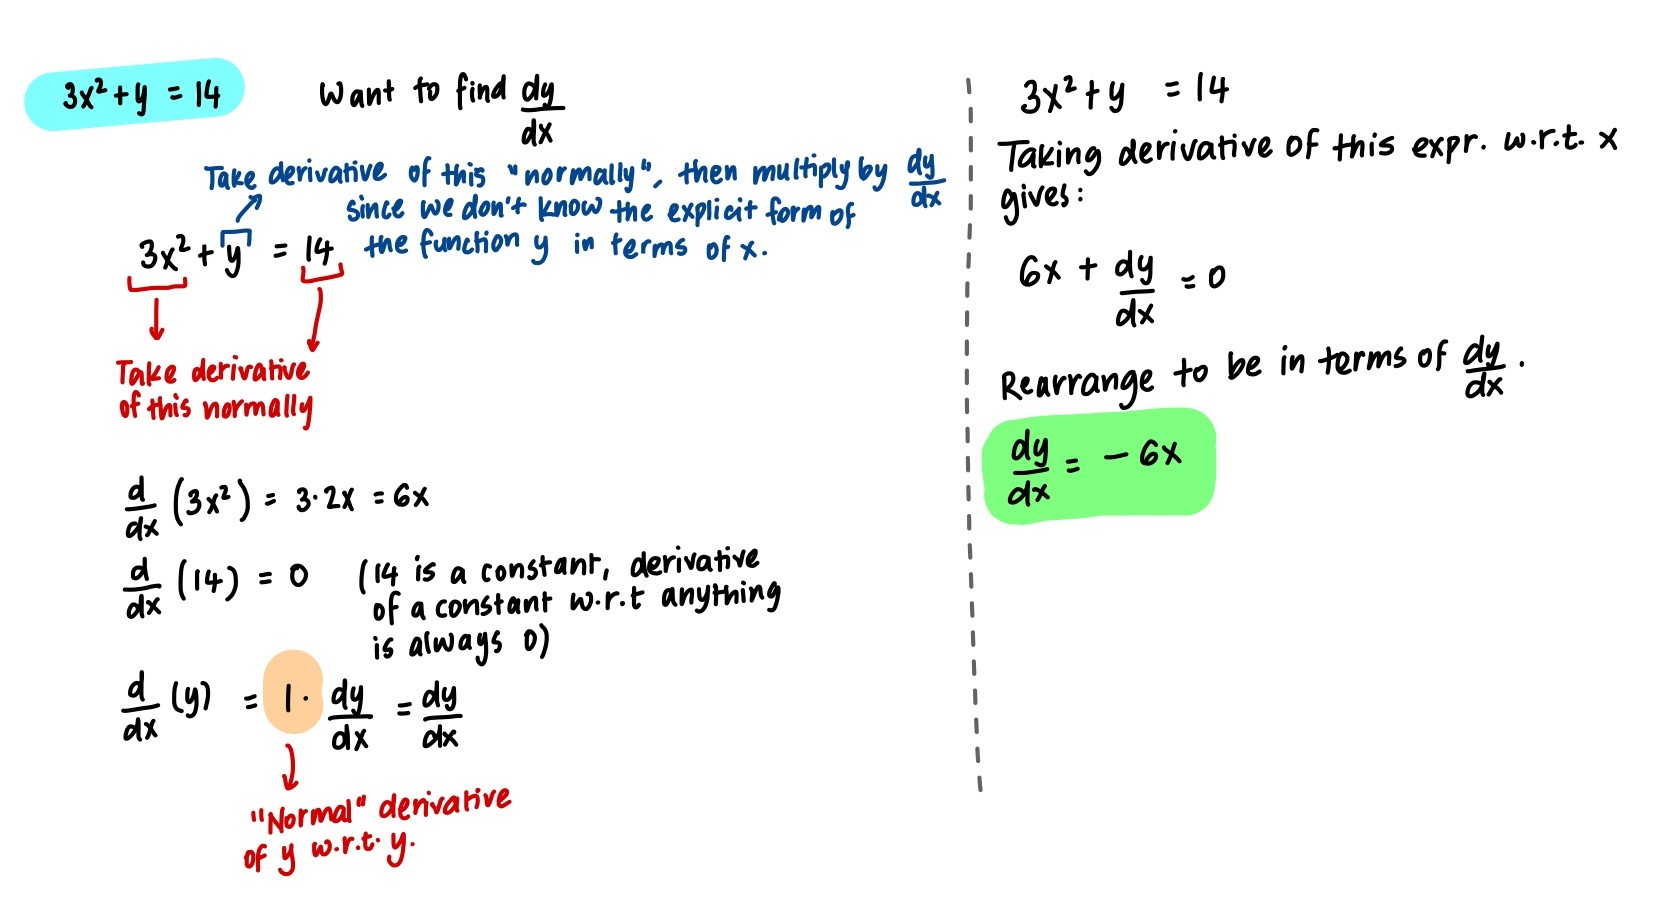
\includegraphics[width=0.85 \linewidth]{Q1.jpg}
        \label{fig:Q1}
    \end{figure}

    \item $x^2y^2 = 1$
    \begin{figure}[H]
        \centering
        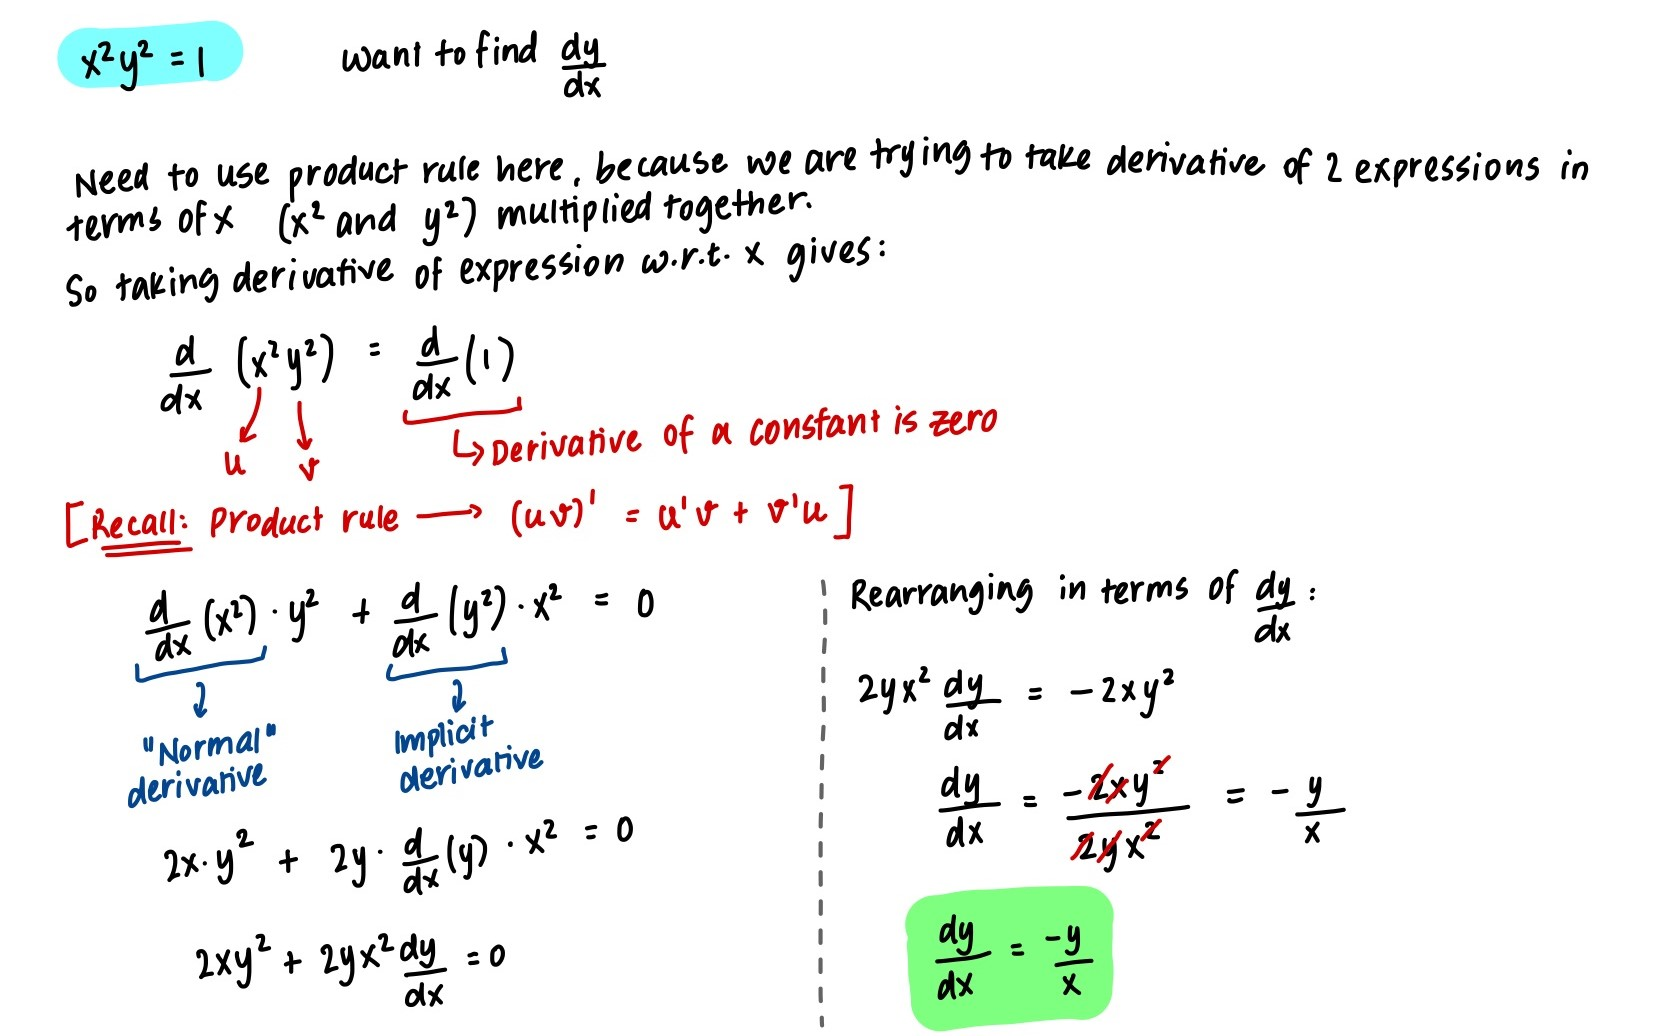
\includegraphics[width=0.85\linewidth]{Q2.jpg}
        \label{fig:Q2}
    \end{figure}

    \item $\sqrt{y} + xy^2 = 15$
    \begin{figure}[H]
        \centering
        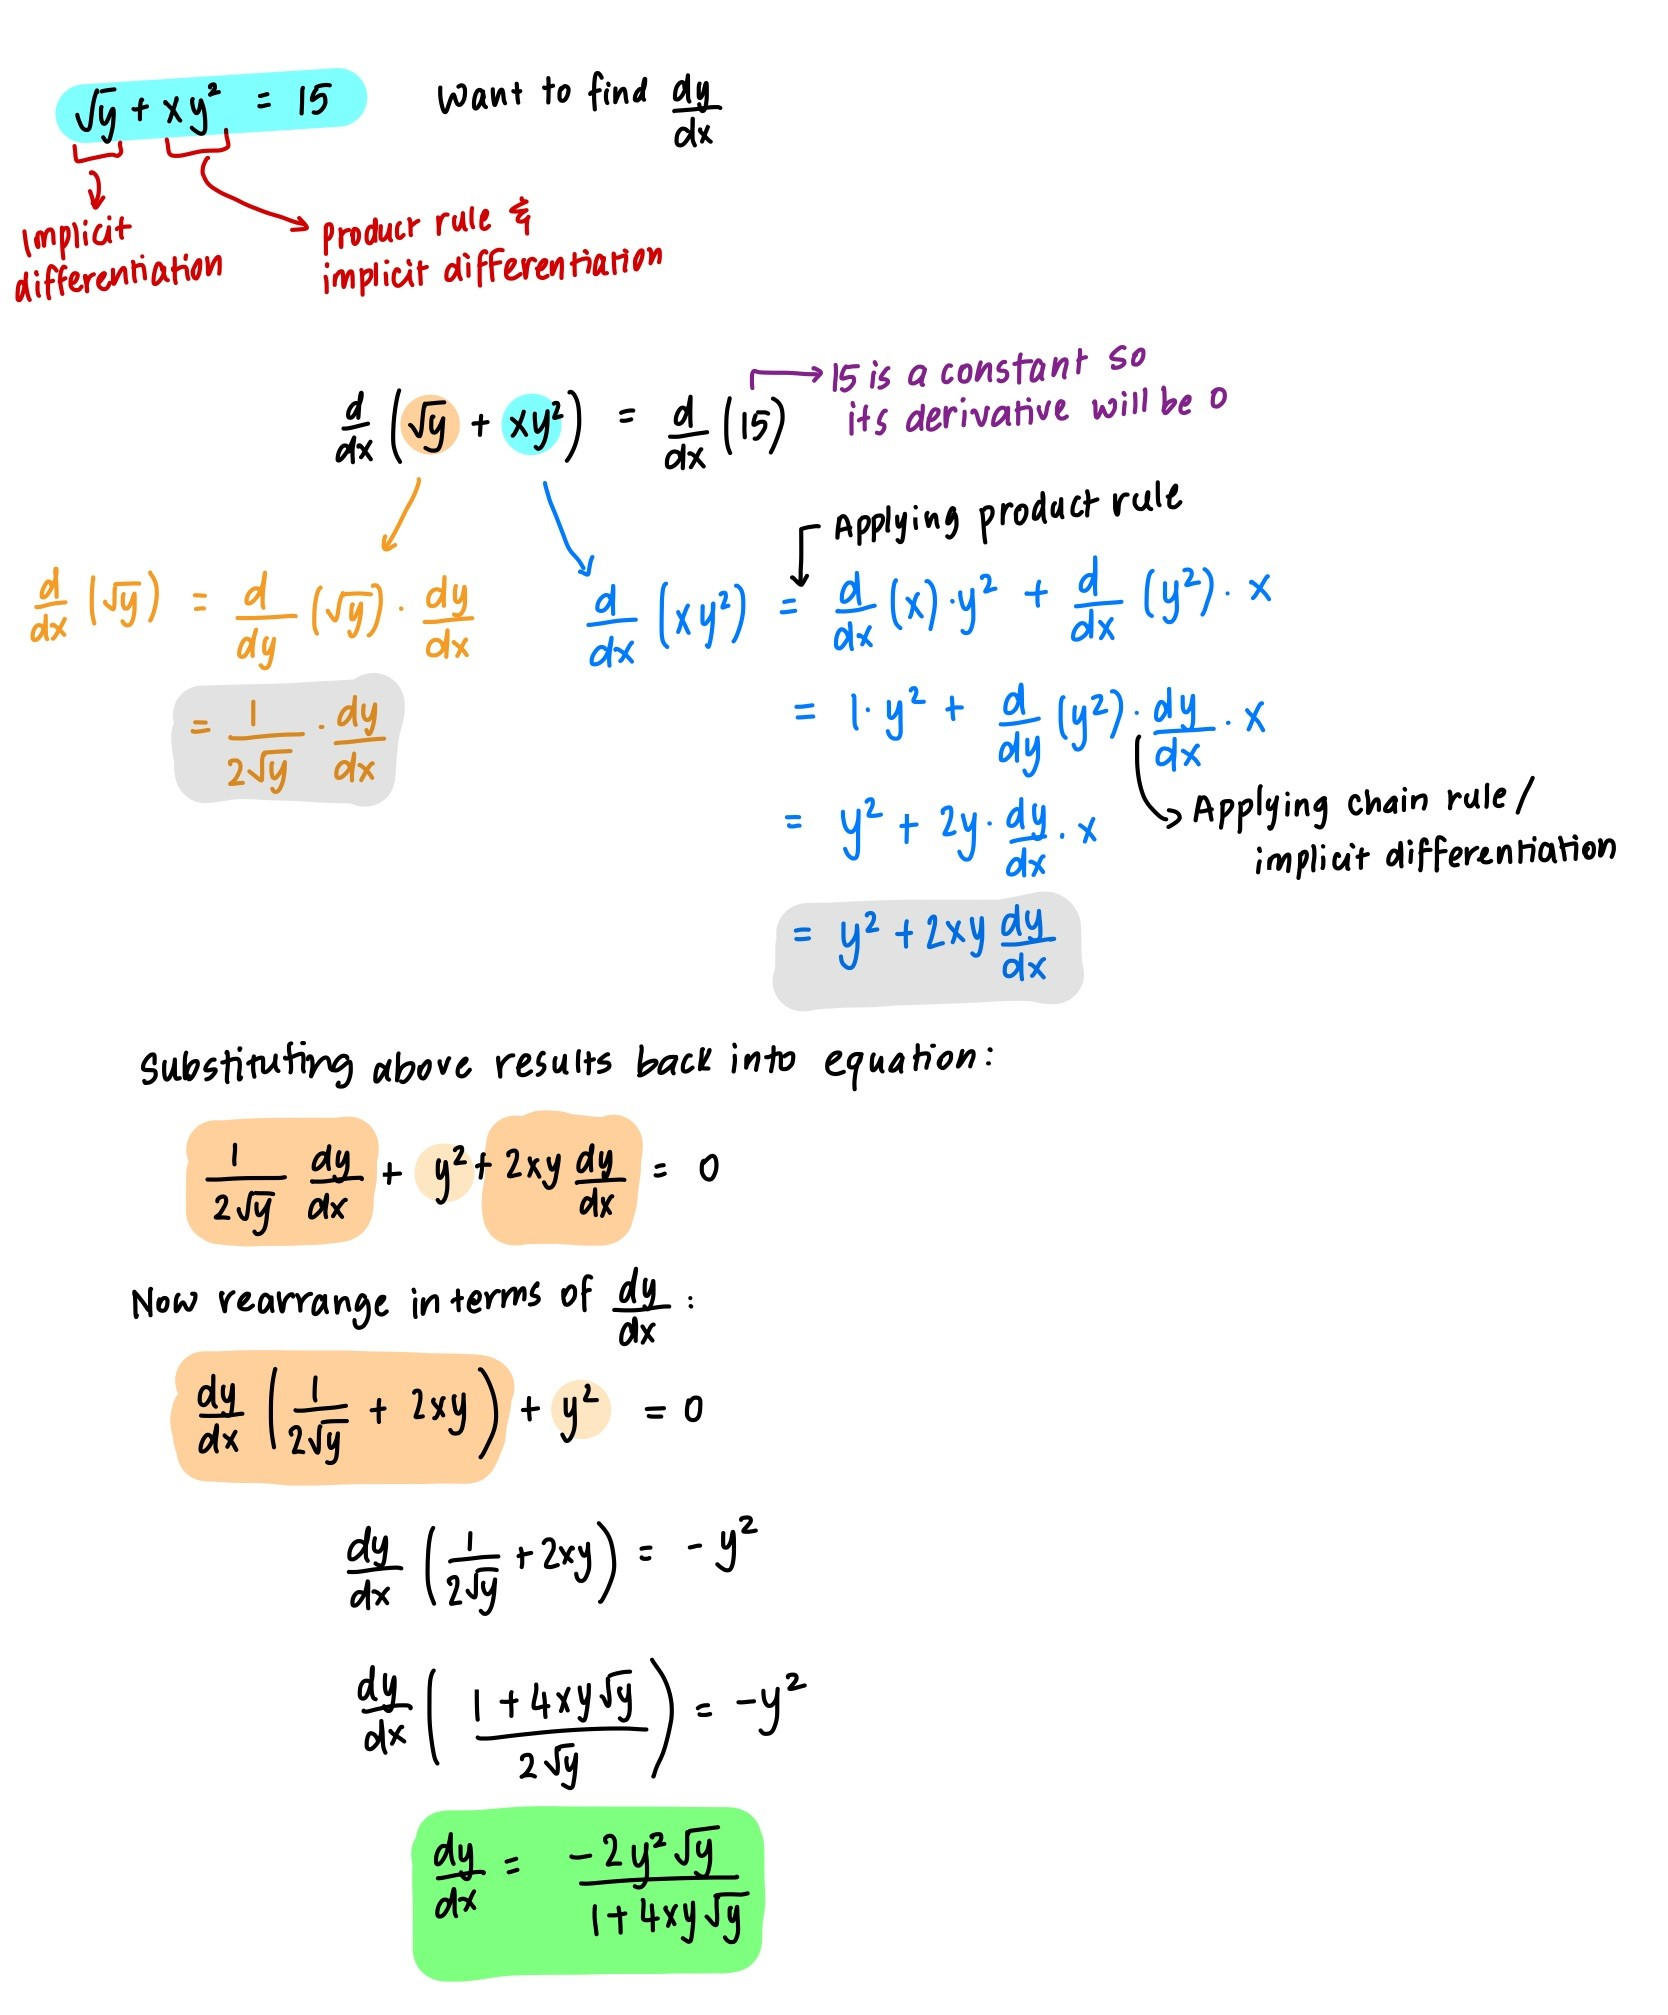
\includegraphics[width=\linewidth]{Q3.jpg}
        \label{fig:Q3}
    \end{figure}
    
    \item $(x-y)^2 = x + y - 1$
    \begin{figure}[H]
        \centering
        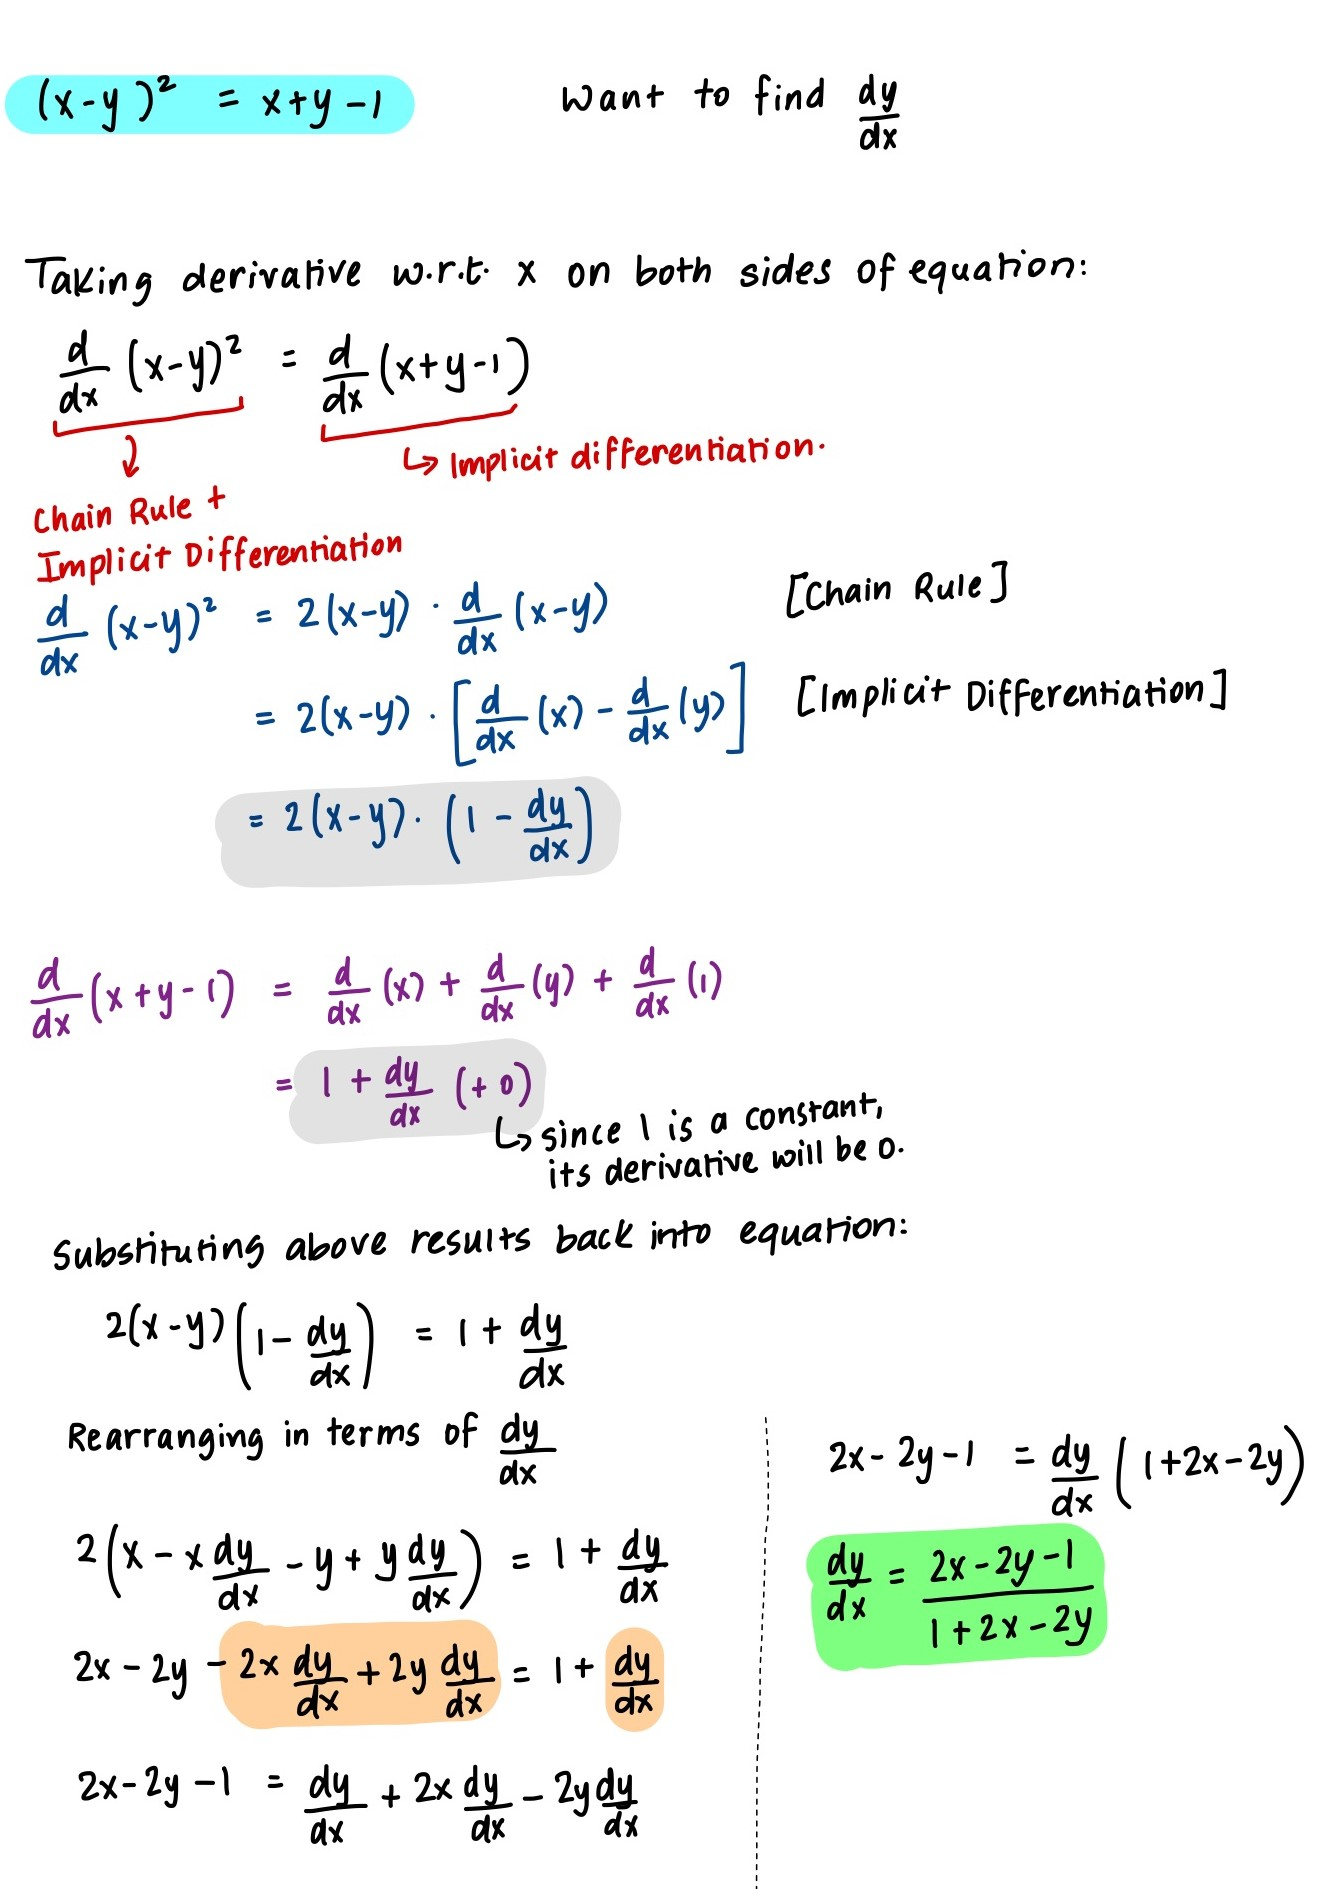
\includegraphics[width=0.85\linewidth]{Q4.jpg}
        \label{fig:Q4}
    \end{figure}

    \item $ \cos^2 x + \cos^2 y = \cos( 2x + 2y )$ 
    \begin{figure}[H]
        \centering
        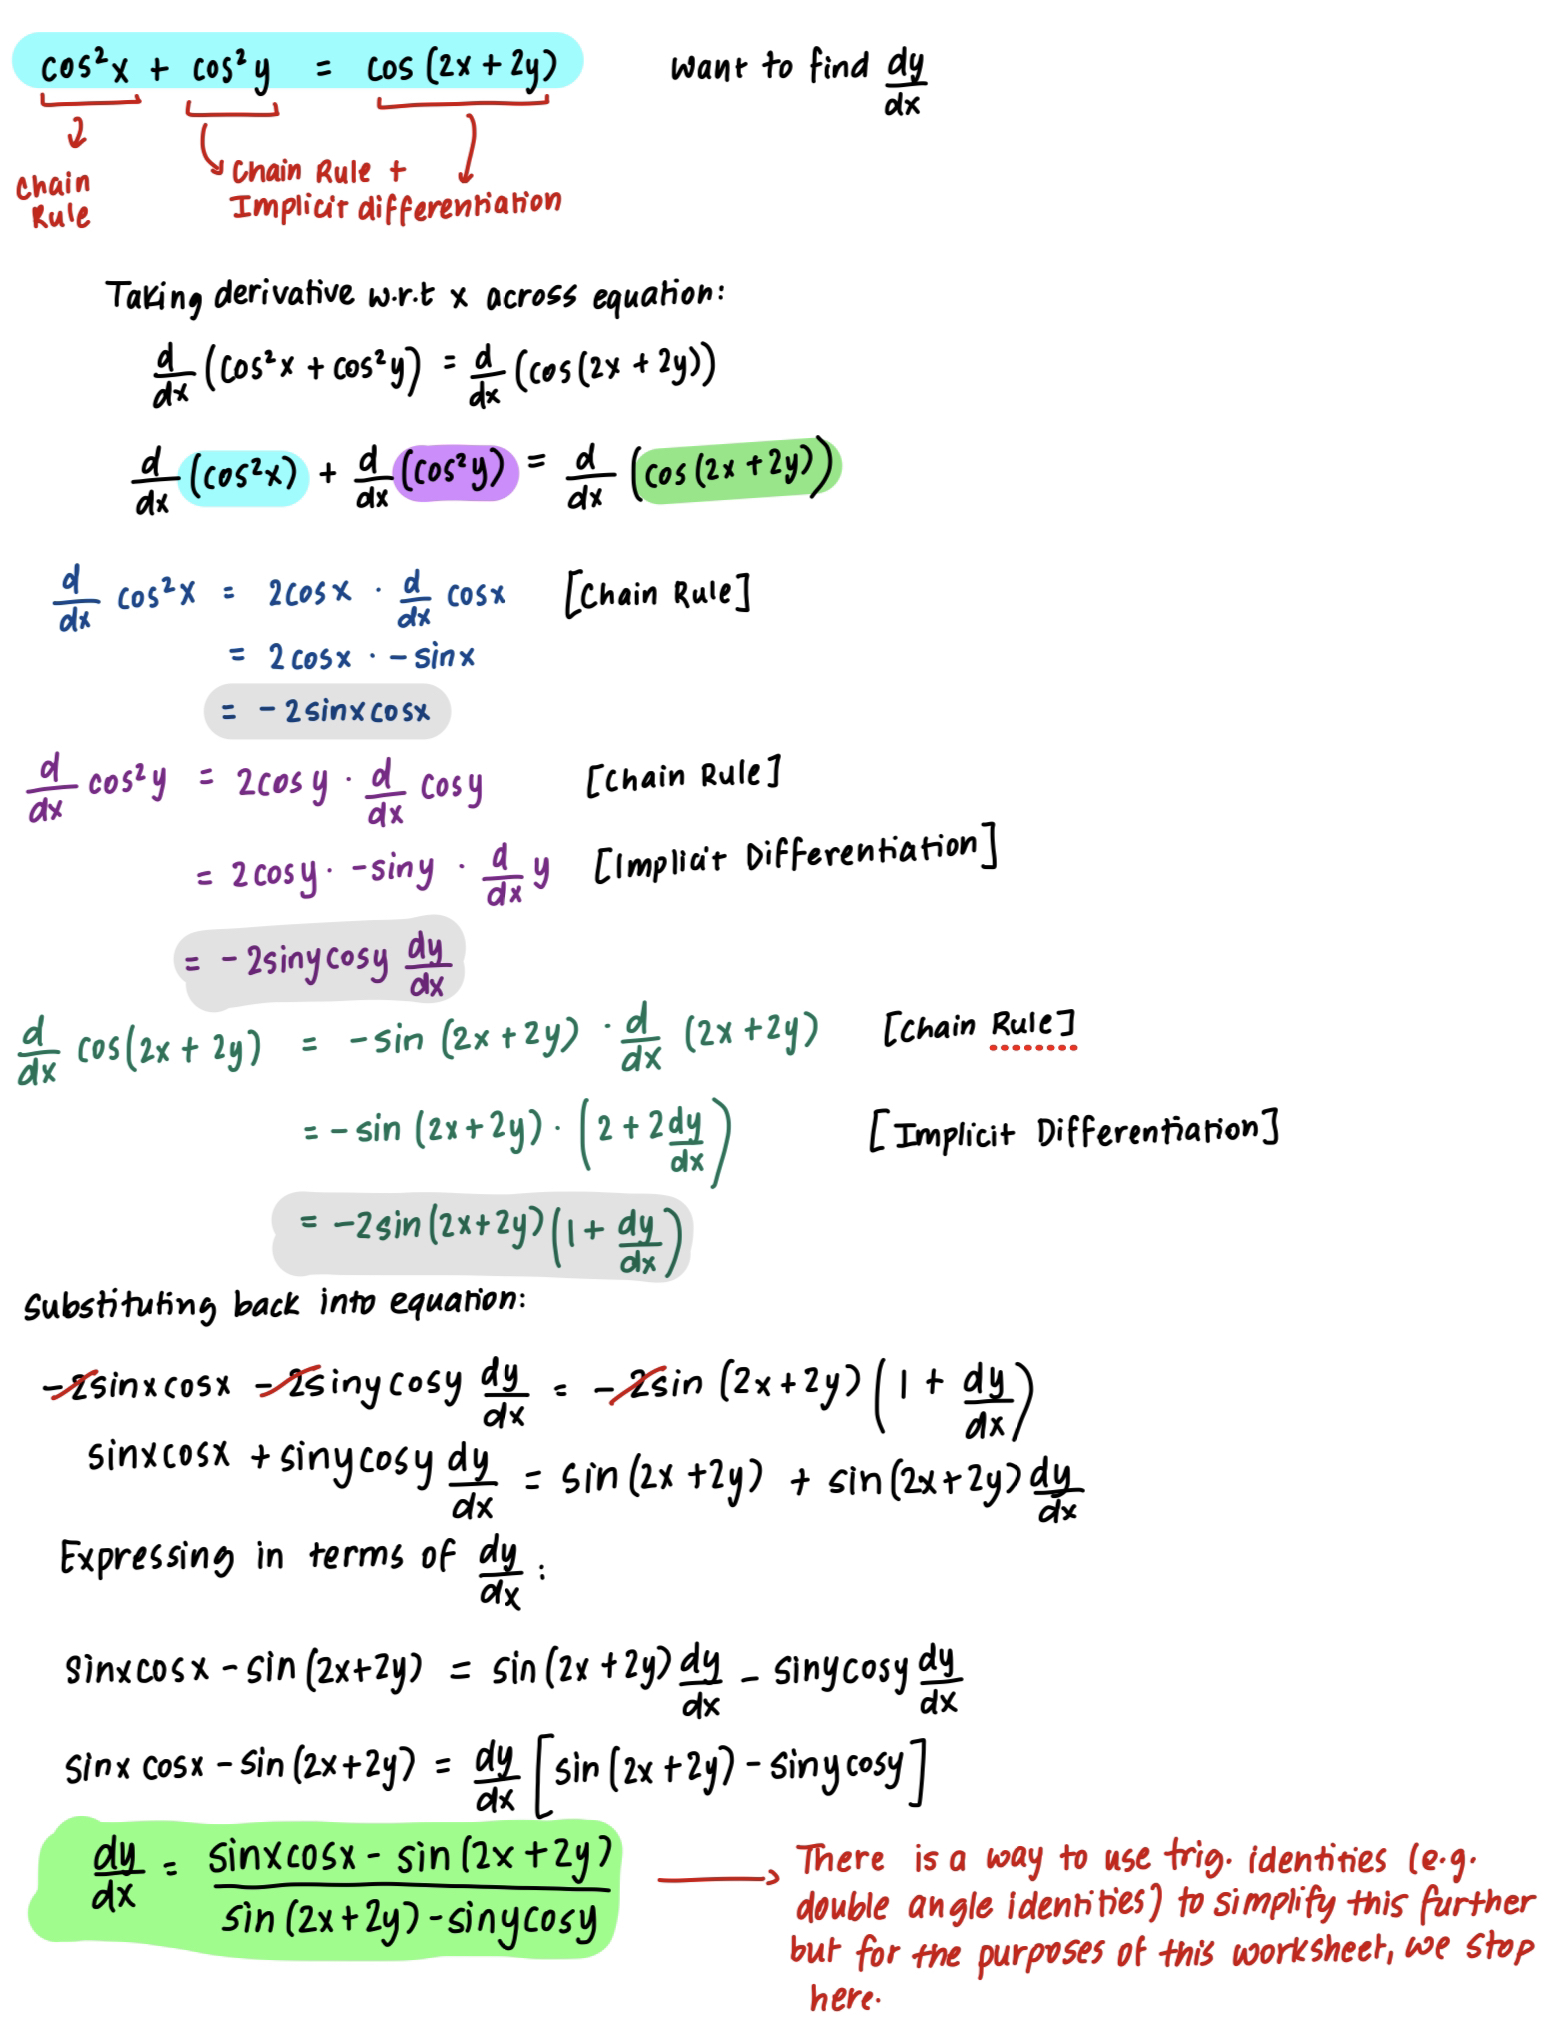
\includegraphics[width=0.95\linewidth]{Q5.jpg}
        \label{fig:Q5}
    \end{figure}

    \item $x = \sqrt{\tan y^2}$
    \begin{figure}[H]
        \centering
        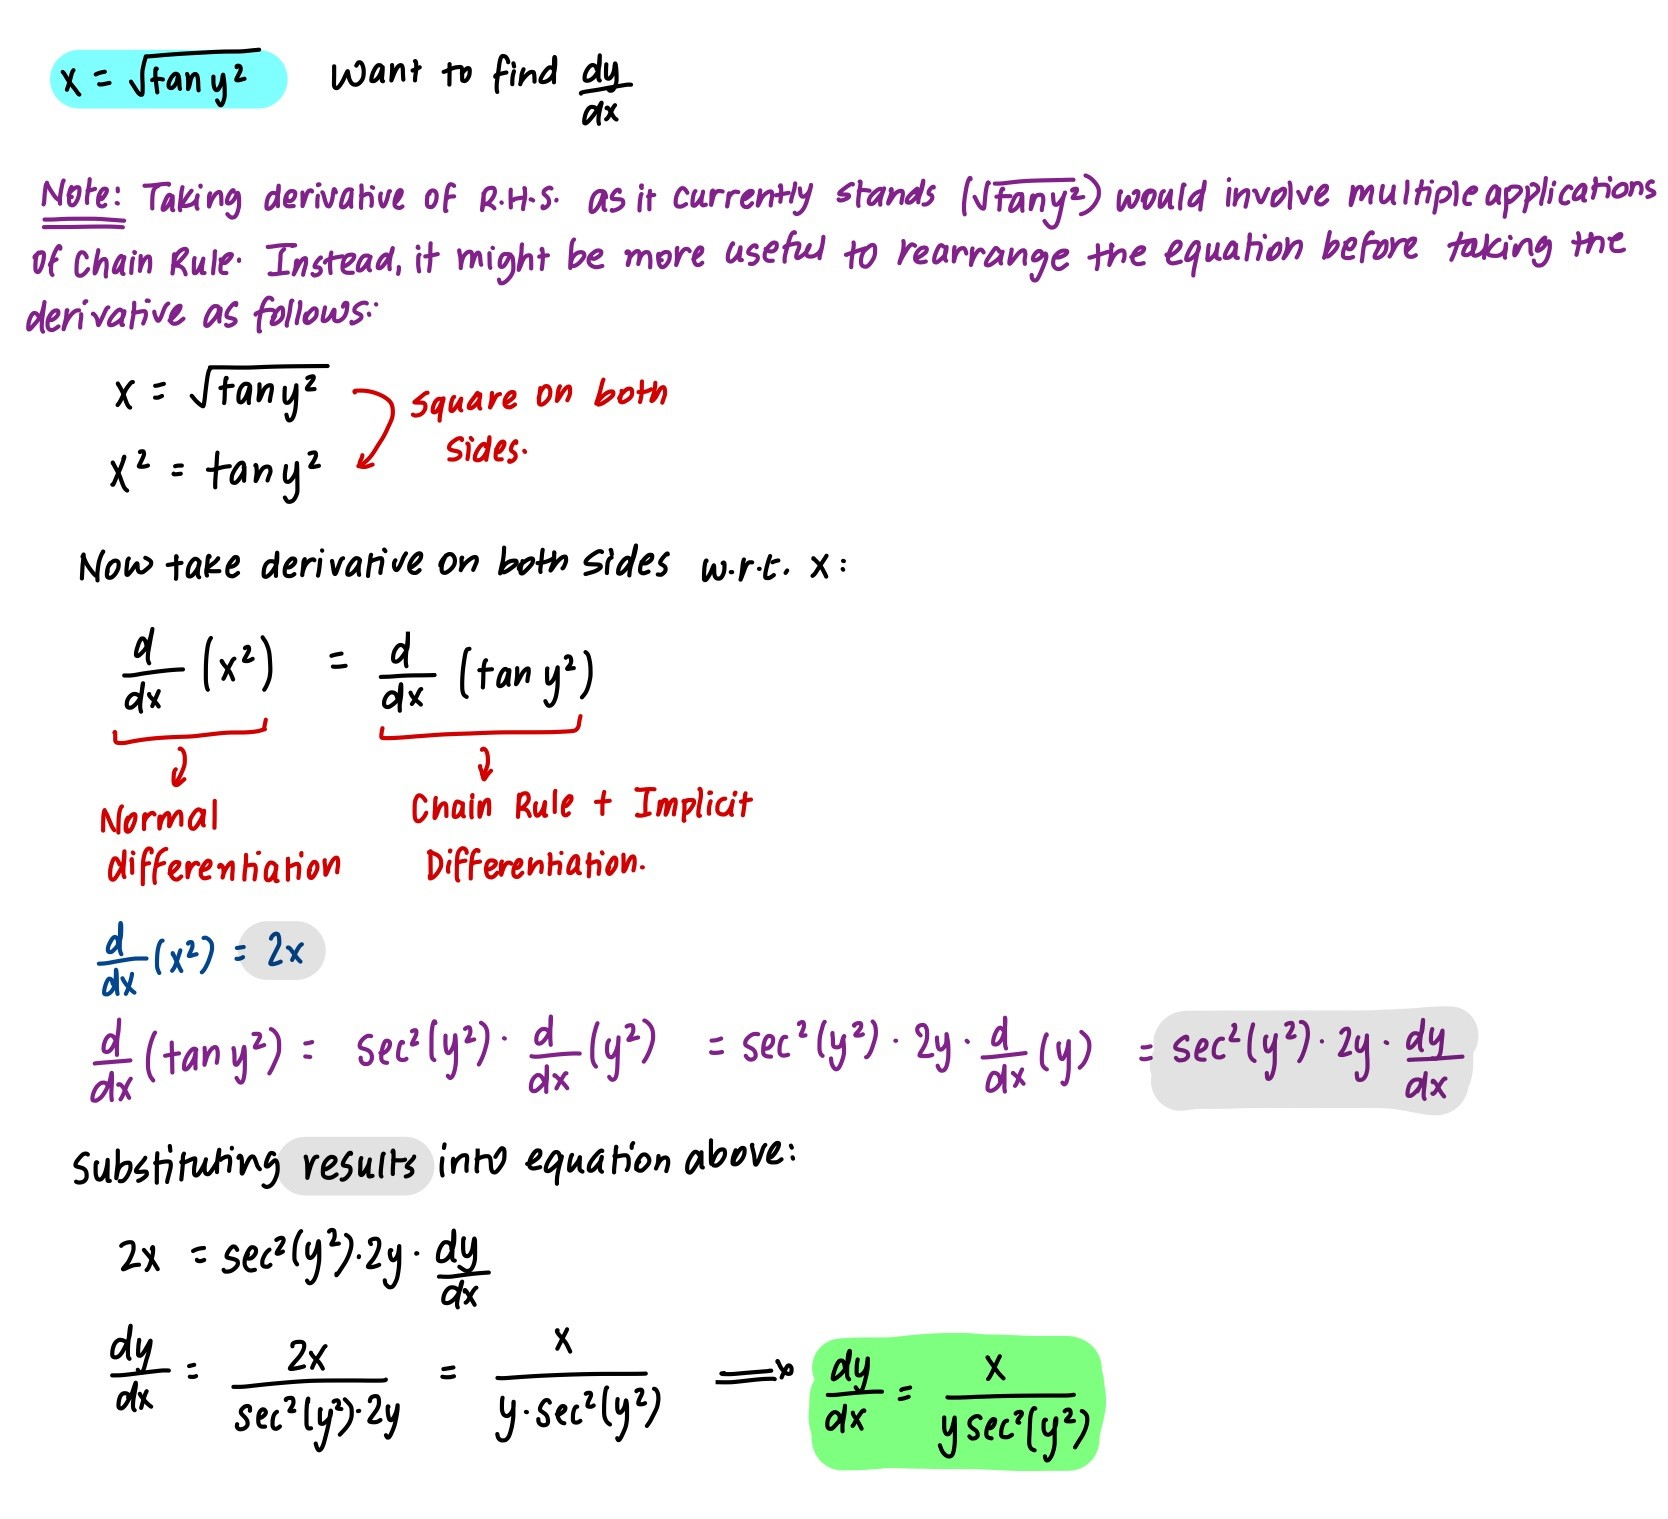
\includegraphics[width=0.95\linewidth]{Q6.jpg}
        \label{fig:Q6}
    \end{figure}

\end{enumerate}
Note: Word Problems continue on the next page. 

\pagebreak
\subsection*{Word Problems}
\href{https://www.rit.edu/academicsuccesscenter/sites/rit.edu.academicsuccesscenter/files/documents/math-handouts/C4_ImplicitDifferentiationandRelatedRates_BP_5_6_19.pdf}{Source}
\begin{enumerate}
    \item Find the equation of the tangent line to the curve defined by $2x^3-5y^2=5$ at the point $(2, -1)$.
     \begin{figure}[H]
        \centering
        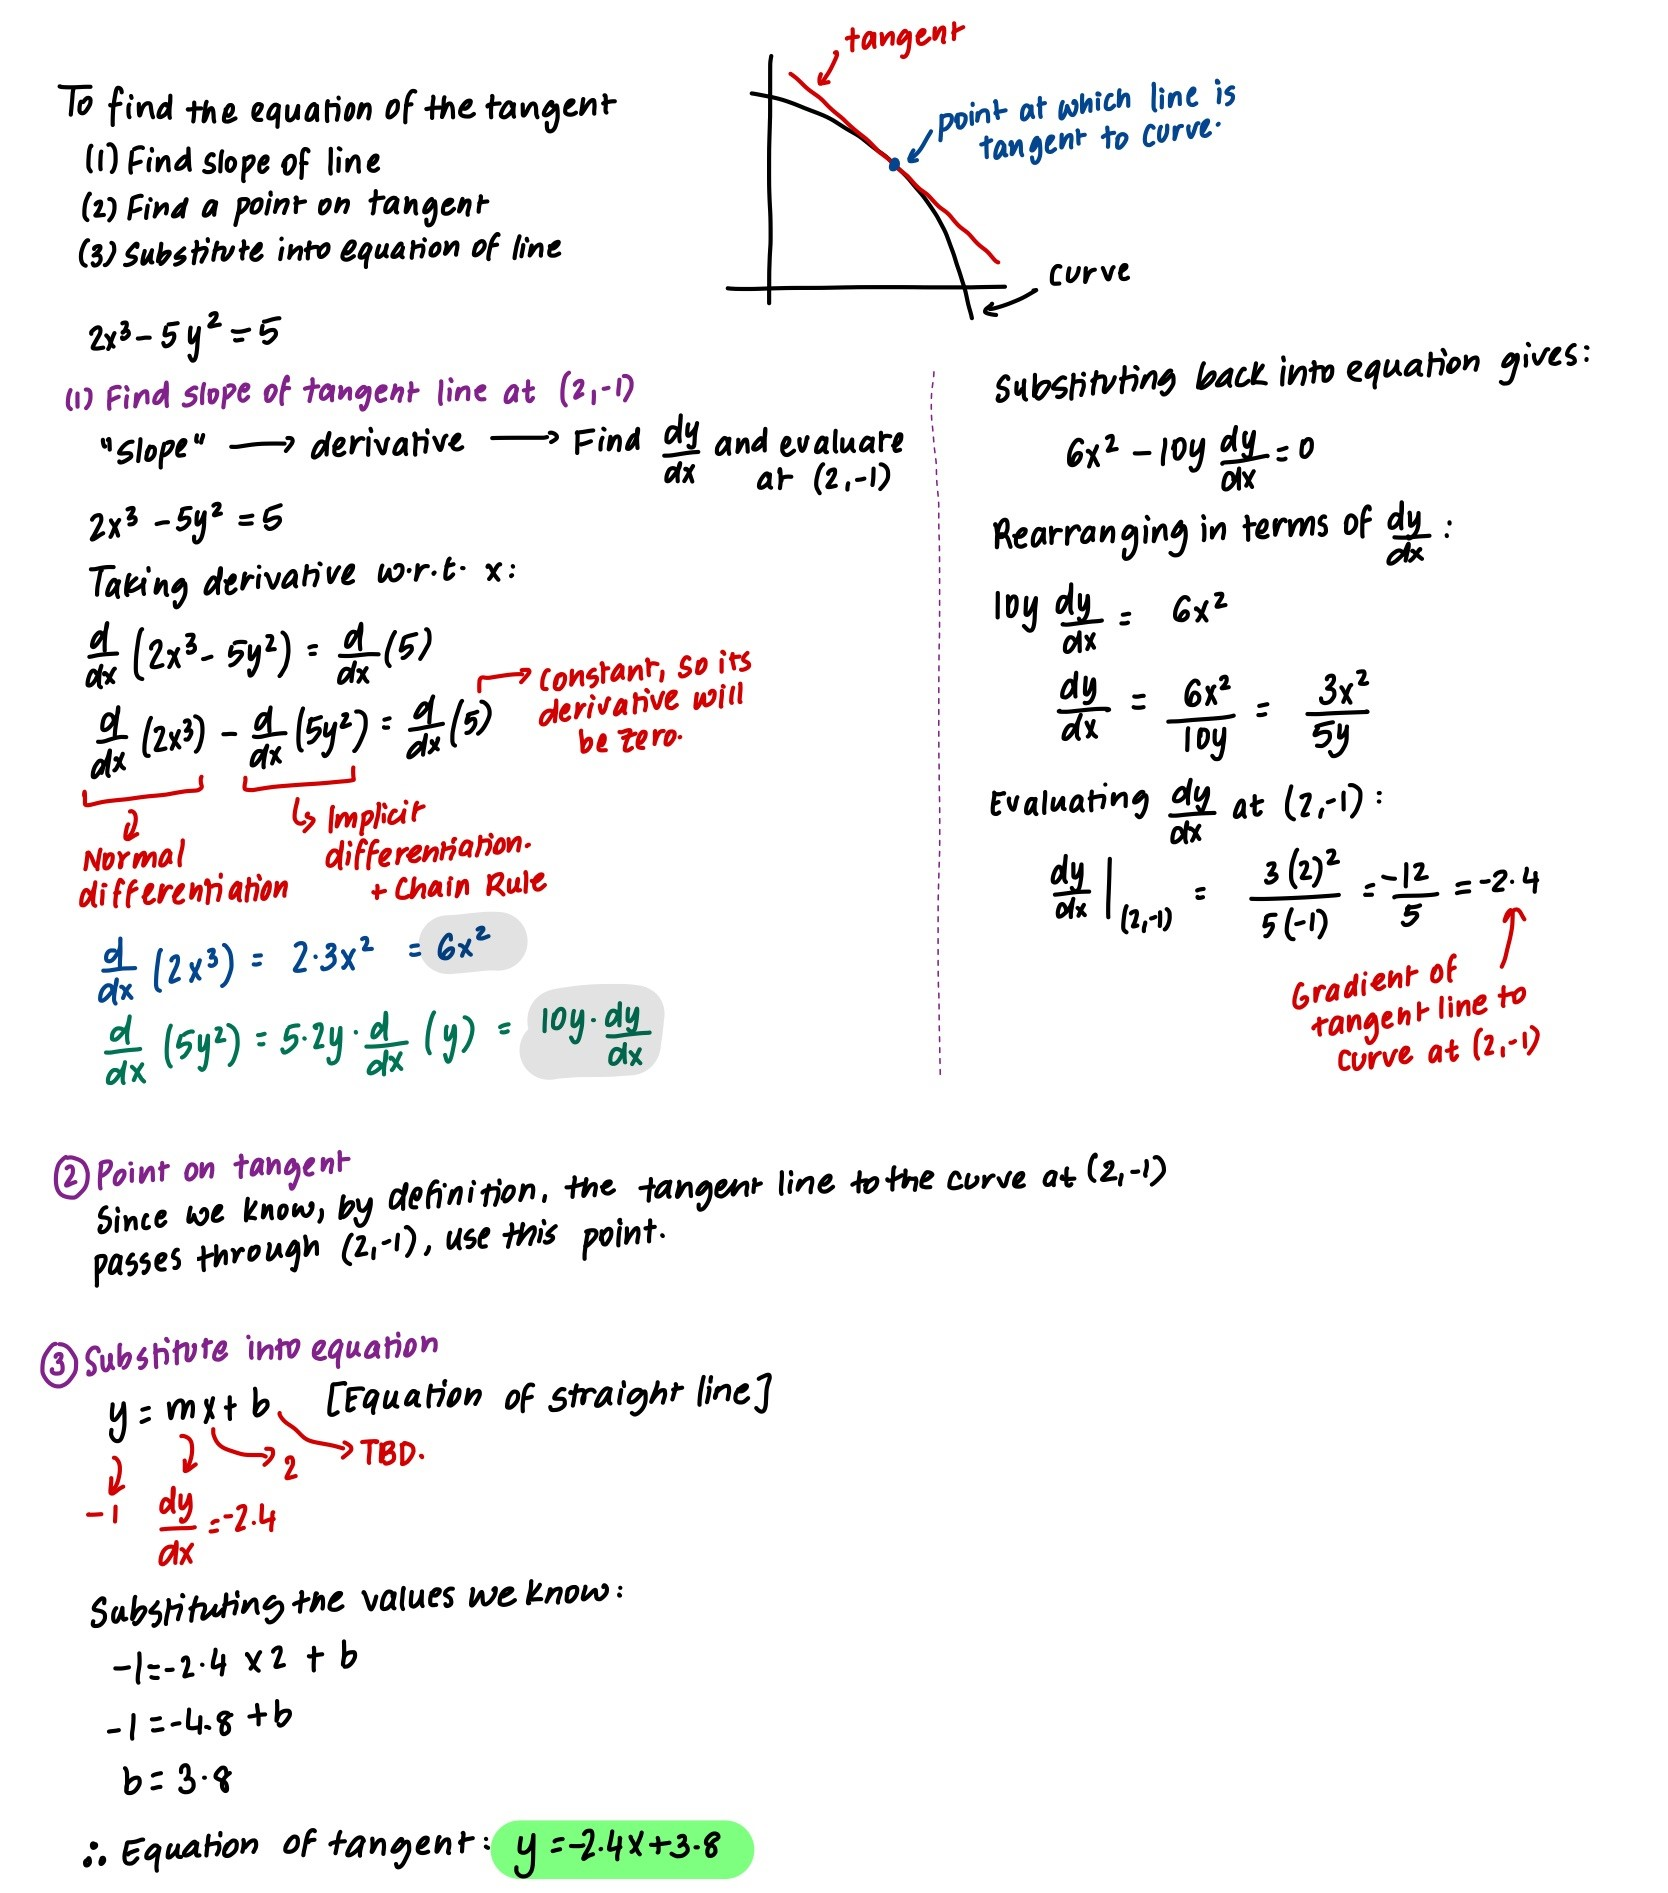
\includegraphics[width=\linewidth]{Q7.jpg}
        \label{fig:Q7}
    \end{figure}

    \item Find the equation of the tangent line to the curve defined by $y^2 + 2xy + 4 = 0$ at the point $(2, -2)$
     \begin{figure}[H]
        \centering
        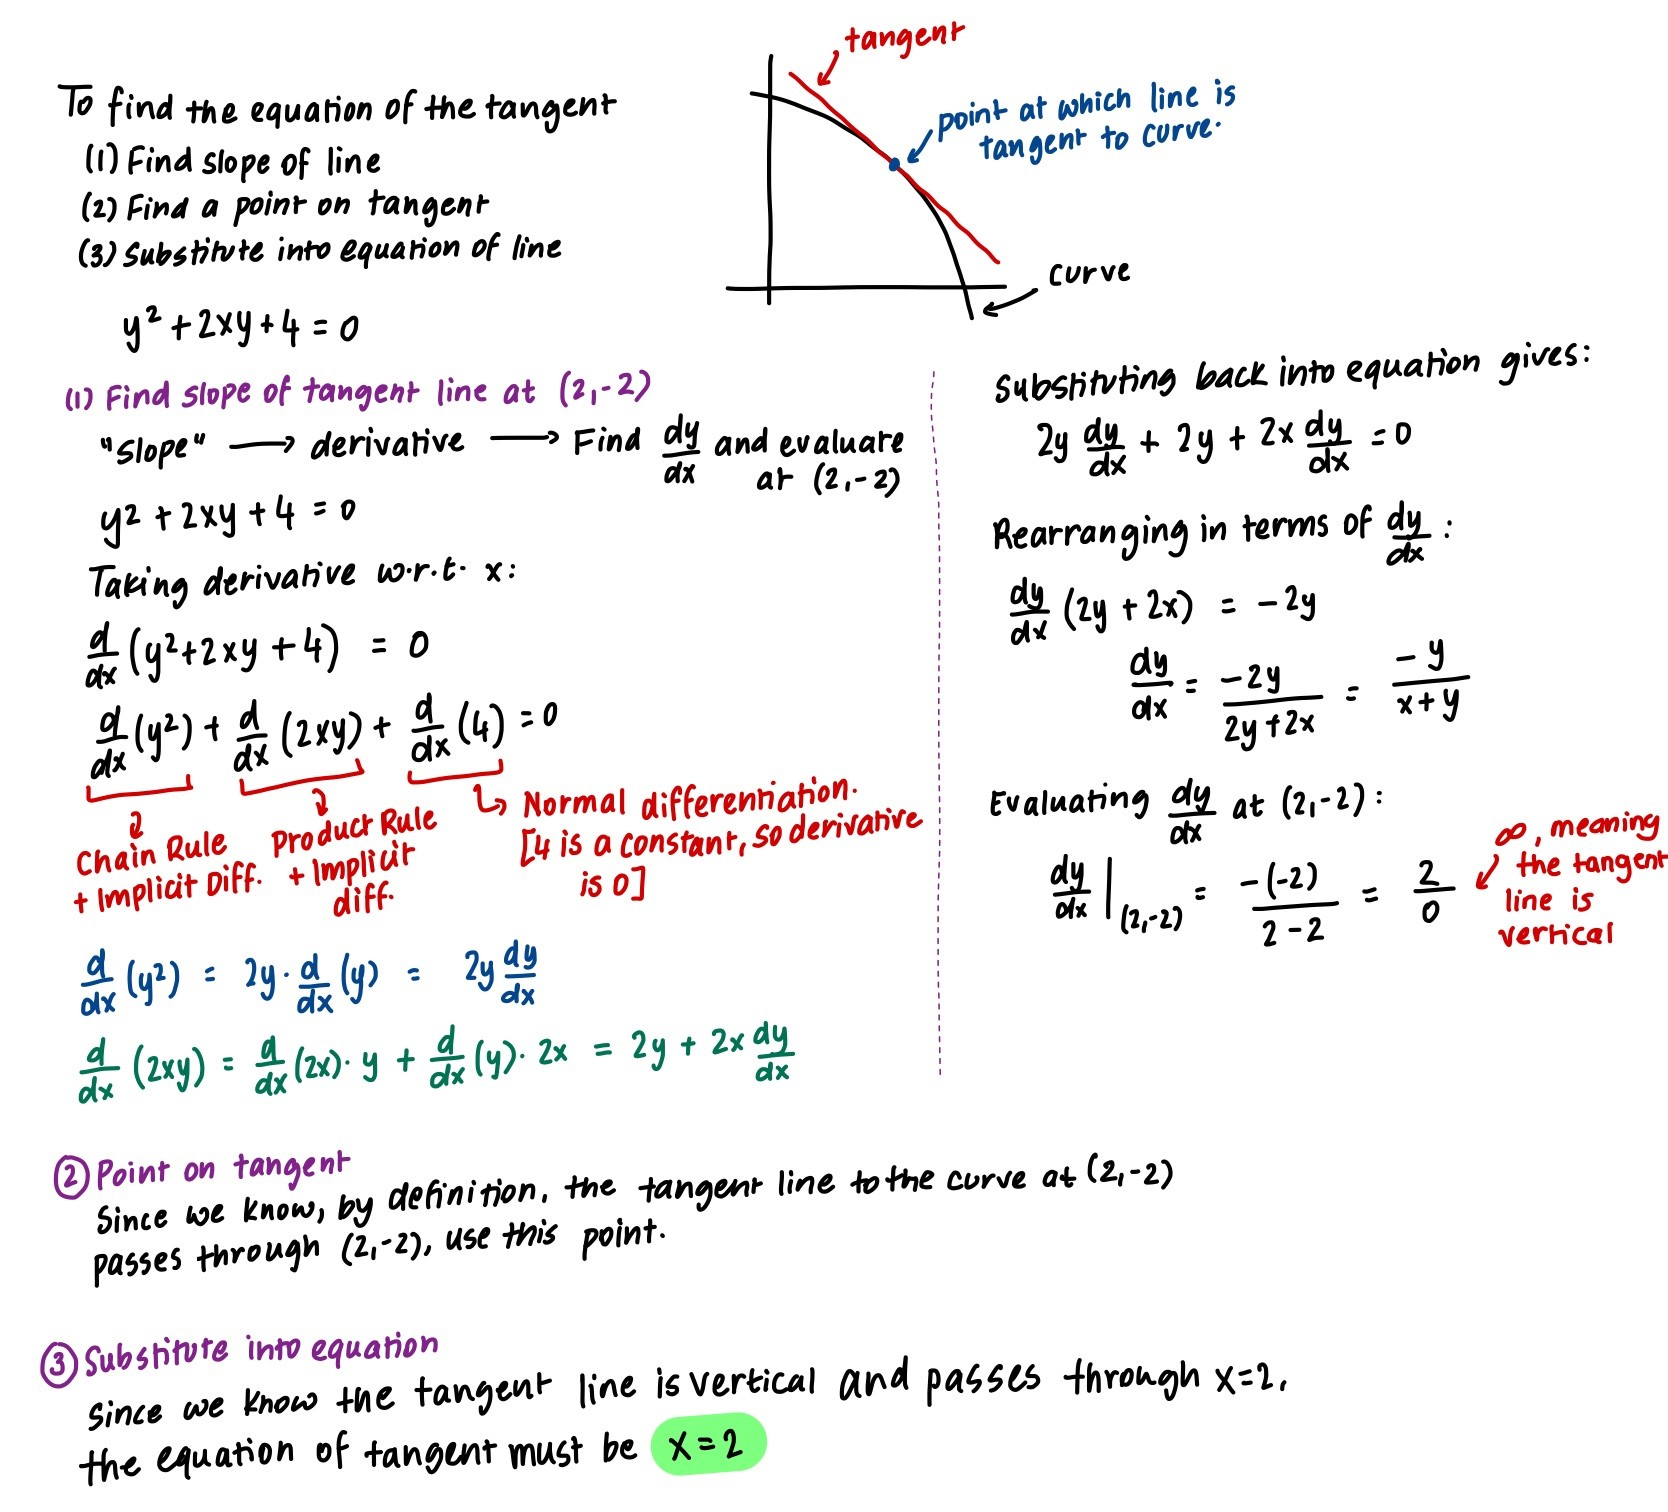
\includegraphics[width=\linewidth]{Q8.jpg}
        \label{fig:Q8}
    \end{figure}
    
\end{enumerate}

\end{document}
